\section{Auswertung}
\label{sec:Auswertung}

\subsection{Aufladeprozess eines Kondensators}
%TODO: Gleichung
Die Messwerte, die während des Aufladeprozesses des Kondensators aufgenommen werden, werden in einem Plot aufgetragen.
Dabei wird GLEICHUNG umgeformt und logarithmisiert, um mittels linearer Regression eine Gerade der Form

%Aufladen
\begin{equation}
    ln\bigg(1  - \frac{U_C}{U_0}\bigg) = -ax + b_1
\end{equation}

über die Messwerte zu legen. Dabei beträgt die Maximalspannung $U_0=15,\~2$V. Die gemessenen Daten sind in \autoref{tab:aufladen} zu finden und der geplottete Graph in \autoref{fig:aufladen}.

\begin{table}[!htp]
\centering
\caption{Messwerte des Aufladevorgangs.}
\label{tab:aufladen}
\begin{tabular}{S[table-format=1.2] S[table-format=2.1]}
\toprule
{$t$ / ms} & {$U$ / V} \\
\midrule
0.28 & 2.0 \\
0.40 & 3.2 \\
0.48 & 4.0 \\
0.64 & 5.2 \\
0.76 & 6.2 \\
0.88 & 7.0 \\
1.04 & 8.0 \\
1.24 & 9.0 \\
1.36 & 9.6 \\
1.52 & 10.2 \\
1.84 & 11.2 \\
2.04 & 12.0 \\
2.20 & 12.4 \\
\bottomrule
\end{tabular}
\end{table}

\begin{figure}
    \centering
    \includegraphics{build/plot-aufladen.pdf}
    \caption{Plot der Messdaten des Aufladevorgangs.}
    \label{fig:aufladen}
\end{figure}

Mittels Python 3.7.0 bestimmen sich folgende Werte für die Koeffizienten:

\begin{center}
    $a = (800 \pm 8) \frac{1}{\symup{s}}$

    $b_1 = 0,\~08 \pm 0,\~01$.
\end{center}

Mit der Relation

\begin{center}
    $a = \frac{1}{RC}$
\end{center}

folgt direkt

\begin{center}
    $RC = (1,\~26 \pm 0,\~01) \cdot 10^{-3}$ s.
\end{center}

\subsection{Angelegtes Sinussignal mit variabler Frequenz}

Die Messwerte, die während der Messung mit einem angelegtem Sinussignal aufgenommen werden, sind in \autoref{tab:var-freq} zu sehen.
Zur Verschaulichung werden diese Werte in zwei Diagrammen aufgetragen, wobei die $f$-Achsen jeweils logarithmisch skaliert sind.

\begin{table}[!htp]
\centering
\caption{Daten der Messung der Amplitude und Phasenverschiebung bei verschiedenen Frequenzen.}
\label{tab:var-freq}
\begin{tabular}{S[table-format=5.0] S[table-format=2.2] S[table-format=5]}
\toprule
{$f$ / Hz} & {$U$ / V} & {$a$ / µs} \\
\midrule
10 & 15.0 & -8600 \\
20 & 14.6 & -1200 \\
30 & 14.4 & 40 \\
40 & 14.0 & 600 \\
50 & 13.8 & 860 \\
60 & 13.4 & 940 \\
70 & 12.8 & 900 \\
80 & 12.4 & 940 \\
90 & 11.9 & 960 \\
100 & 11.5 & 960 \\
200 & 7.76 & 760 \\
300 & 5.64 & 620 \\
400 & 4.44 & 500 \\
500 & 3.60 & 420 \\
600 & 2.96 & 360 \\
700 & 2.56 & 310 \\
800 & 2.24 & 280 \\
900 & 2.00 & 250 \\
1000 & 1.82 & 230 \\
2000 & 1.00 & 120 \\
3000 & 0.76 & 82 \\
4000 & 0.56 & 61 \\
5000 & 0.48 & 49 \\
6000 & 0.38 & 41 \\
7000 & 0.26 & 35 \\
8000 & 0.23 & 31 \\
9000 & 0.21 & 29 \\
10000 & 0.19 & 25 \\
\bottomrule
\end{tabular}
\end{table}

Zunächst wird das Amplitudenverhältnis $\frac{U_C}{U_0}$ gegen die Kreifrequenz $\omega = 2 \pi f$ aufgetragen. Darüber wird ein Fit der Form

\begin{equation}
    \frac{U_C}{U_0} = \frac{1}{\sqrt{ b_2 + \omega^2 \cdot (RC)^2 }}
\end{equation}

gelegt. Dieser Plot ist in \autoref{fig:amplitude} zu sehen.

\begin{figure}
    \centering
    \includegraphics{build/plot-amplitude.pdf}
    \caption{Plot der Messdaten der Amplitude in Frequnzabhängigkeit.}
    \label{fig:amplitude}
\end{figure}

\begin{table}[!htp]
\centering
\caption{Daten der Messung der Amplitude und Phasenverschiebung bei verschiedenen Frequenzen.}
\label{tab:var-freq}
\begin{tabular}{S[table-format=5.0] S[table-format=2.2] S[table-format=5]}
\toprule
{$f$ / Hz} & {$U$ / V} & {$a$ / µs} \\
\midrule
10 & 15.0 & -8600 \\
20 & 14.6 & -1200 \\
30 & 14.4 & 40 \\
40 & 14.0 & 600 \\
50 & 13.8 & 860 \\
60 & 13.4 & 940 \\
70 & 12.8 & 900 \\
80 & 12.4 & 940 \\
90 & 11.9 & 960 \\
100 & 11.5 & 960 \\
200 & 7.76 & 760 \\
300 & 5.64 & 620 \\
400 & 4.44 & 500 \\
500 & 3.60 & 420 \\
600 & 2.96 & 360 \\
700 & 2.56 & 310 \\
800 & 2.24 & 280 \\
900 & 2.00 & 250 \\
1000 & 1.82 & 230 \\
2000 & 1.00 & 120 \\
3000 & 0.76 & 82 \\
4000 & 0.56 & 61 \\
5000 & 0.48 & 49 \\
6000 & 0.38 & 41 \\
7000 & 0.26 & 35 \\
8000 & 0.23 & 31 \\
9000 & 0.21 & 29 \\
10000 & 0.19 & 25 \\
\bottomrule
\end{tabular}
\end{table}

Nach dieser Methode berechnet sich die Zeitkonstante mittels Python 3.7.0 als

\begin{centering}
    $RC = (1,\~36 \pm 0,\~02) \cdot 10^{-3} $s

    $b_2 = 1,\~049 \pm 0,\~006$
\end{centering}

%TODO: Gleichung
Um die Phasenverschiebung mittels der Daten in \autoref{tab:var-freq} zu errechnen wird GLEICHUNG verwendet.
Diese Daten werden ebenfalls geplottet und über diese wird ein Fit der Form

%Phasenverschiebung
\begin{equation}
    \phi = \arctan (-RC \cdot \omega + b_3)
\end{equation}

gelegt. Das resultierende Diagramm ist in \autoref{fig:phasenverschiebung} zu finden.

\begin{figure}
    \centering
    \includegraphics{build/plot-phasenverschiebung.pdf}
    \caption{Plot der Messdaten der Phasenverschiebung in Frequnzabhängigkeit.}
    \label{fig:phasenverschiebung}
\end{figure}

Ebenfalls mittels Pyhton 3.7.0 ermittelt sich die Koeffizienten mit dieser Methode als

\begin{center}
    $RC = (1,\~33 \pm 0,\~05) \cdot 10^{-3}$s

    $b_3 = -0,\~17 \pm 0,\~02$.
\end{center}

Mittels der Daten in \autoref{tab:var-freq} wird ebenfalls ein Polarplot erstellt. Dabei wird das Amplitudenverhältnis $\frac{U_C}{U_0}$ radial aufgetragen und die Phasenverschiebung als Winkel.
Zur Bestimmung der Ausgleichsfunktion wird zunächst \eqref{eqn:phasendifferenz} umgekehrt. Dadurch entsteht

\begin{equation}
    \omega(\phi) = -\frac{\tan(\phi)}{RC}.
\end{equation}

Dies wird in \eqref{eqn:zusammenhang} eingesetzt und es entsteht die Ausgleichsfunktion

\begin{equation}
    A(\phi) = \frac{\sin(\phi)}{\tan(\phi)} = \cos(\phi).
\end{equation}

Der damit entstehende Plot ist in \autoref{fig:polar} zu sehen.

\begin{figure}
    \centering
    \includegraphics{build/plot-polar.pdf}
    \caption{Das Amplitudenverhältnis in Abhängigkeit von der Phasenverschiebung.}
    \label{fig:polar}
\end{figure}


\subsection{Überprüfung der Integrationsfunktion des RC-Kreises}

Zunächst wird eine Sinusfunktion in den RC-Kreis gesendet. Es gilt

\begin{equation}
    \int \sin(t) \symup{d}t = cos(t).
\end{equation}

Dieses ist in \autoref{fig:sinus} zu sehen.
Daraufhin wird eine Rechteckfunktion integriert. Dabei sei $f(t)$ die Rechteckfunktion, womit

\begin{equation}
    \int f(t) \symup{d}t = \left\{\begin{array}{ll} 
    t & 0 \leq t \less T \\
    -t & T \leq t \less 2T \\
    \end{array}
    \right.
\end{equation}

gilt. Auch dies ist in \autoref{fig:rechteck} zu sehen.
Zuletzt wird ein Dreieckssignal integriert. Nun sei $g(t)$ die Dreiecksfunktion. Damit gilt

\begin{equation}
    \int g(t) \symup{d}t = \left\{\begin{array}{ll}
    \frac{1}{2} t^2 & 0 \leq t \less T \\
    -\frac{1}{2} t^2 & T \leq t \less 2T \\
    \end{array}
    \right.
    .
\end{equation}

Diese Funktion wird ebenfalls von dem Oszilloskop dargestellt und ist in \autoref{fig:dreieck} zu sehen.

\begin{figure}
    \centering
    \begin{subfigure}{0.32\textwidth}
        \centering
        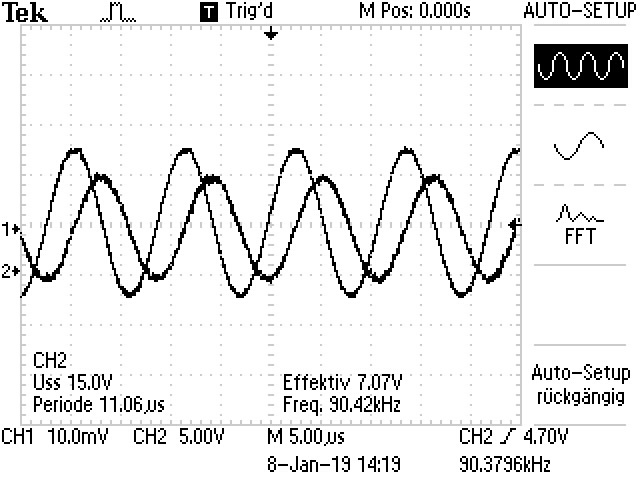
\includegraphics[width=0.95\textwidth]{content/sinus.jpg}
        \caption{Sinussignal.}
        \label{fig:sinus}
    \end{subfigure}
    \begin{subfigure}{0.32\textwidth}
        \centering
        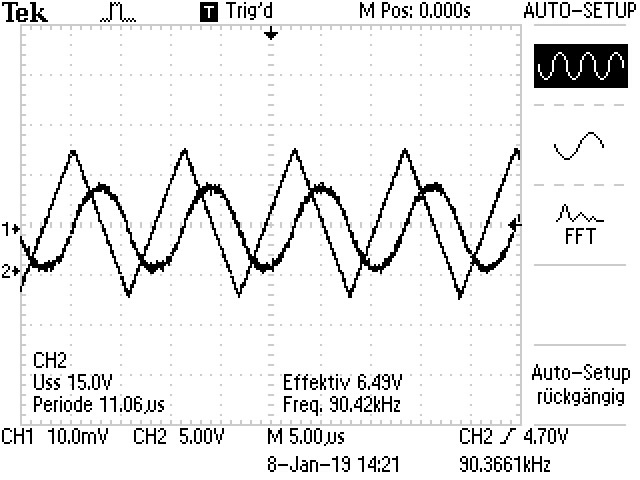
\includegraphics[width=0.95\textwidth]{content/dreieck.jpg}
        \caption{Dreieckssignal.}
        \label{fig:dreieck}
    \end{subfigure}
    \begin{subfigure}{0.32\textwidth}
        \centering
        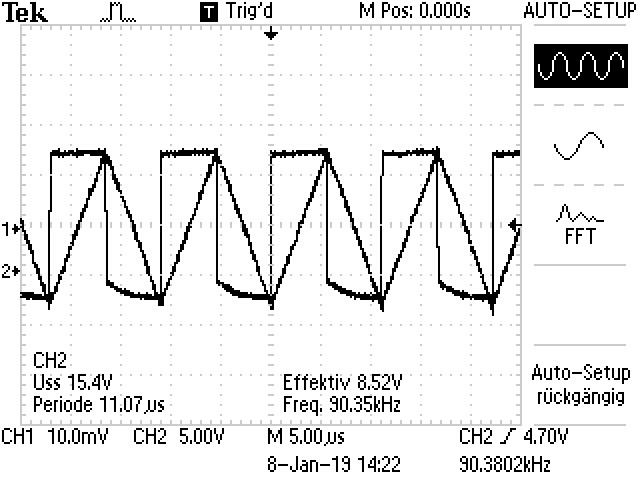
\includegraphics[width=0.95\textwidth]{content/rechteck.jpg}
        \caption{Rechtecksignal.}
        \label{fig:rechteck}
    \end{subfigure}
    \caption{Graphen während der Integrations.}
    \label{fig:integration}
\end{figure}